

\tikzset{every picture/.style={line width=0.75pt}} %set default line width to 0.75pt        

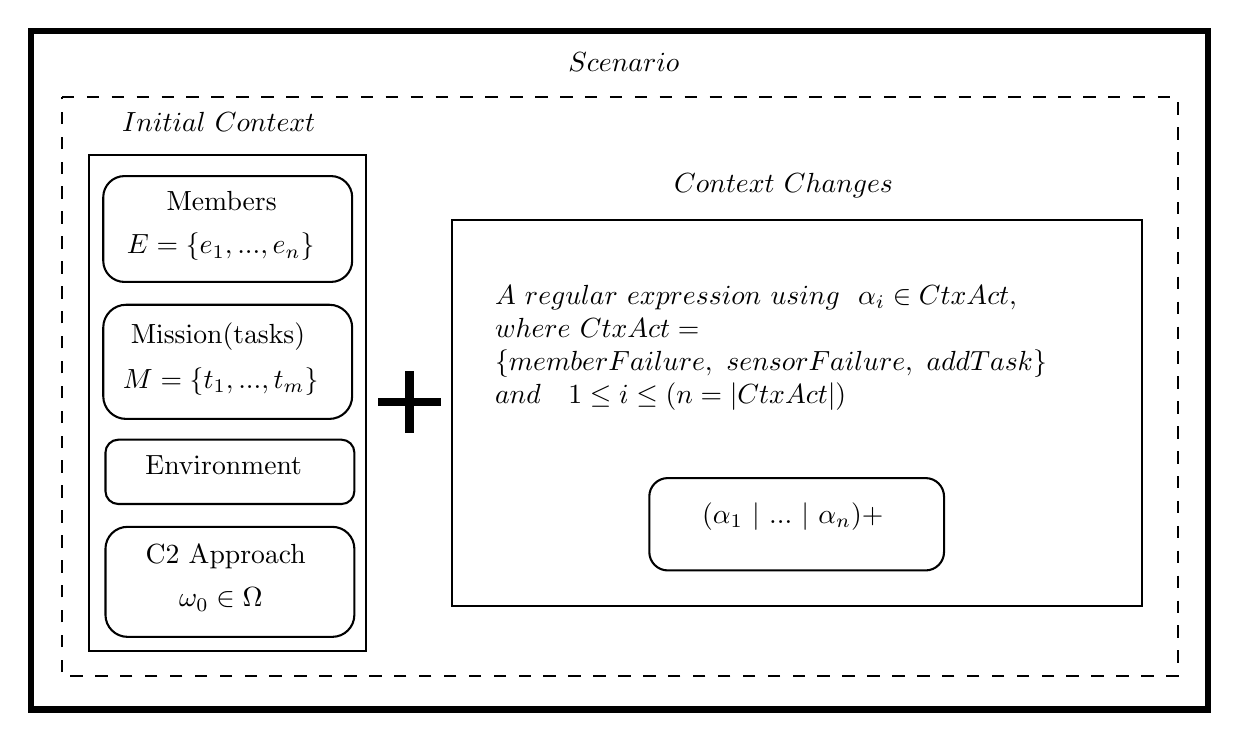
\begin{tikzpicture}[x=0.75pt,y=0.75pt,yscale=-1,xscale=1]
%uncomment if require: \path (0,354); %set diagram left start at 0, and has height of 354

%Rounded Rect [id:dp4190516071959901] 
\draw   (45.48,212.2) .. controls (45.48,208.78) and (48.25,206) .. (51.68,206) -- (159.2,206) .. controls (162.63,206) and (165.4,208.78) .. (165.4,212.2) -- (165.4,230.8) .. controls (165.4,234.22) and (162.63,237) .. (159.2,237) -- (51.68,237) .. controls (48.25,237) and (45.48,234.22) .. (45.48,230.8) -- cycle ;
%Rounded Rect [id:dp916271795400267] 
\draw   (44.41,152) .. controls (44.41,145.92) and (49.34,141) .. (55.41,141) -- (153.34,141) .. controls (159.41,141) and (164.34,145.92) .. (164.34,152) -- (164.34,185) .. controls (164.34,191.08) and (159.41,196) .. (153.34,196) -- (55.41,196) .. controls (49.34,196) and (44.41,191.08) .. (44.41,185) -- cycle ;
%Rounded Rect [id:dp6771464113681669] 
\draw   (44.41,89.2) .. controls (44.41,83.57) and (48.98,79) .. (54.61,79) -- (154.14,79) .. controls (159.77,79) and (164.34,83.57) .. (164.34,89.2) -- (164.34,119.8) .. controls (164.34,125.43) and (159.77,130) .. (154.14,130) -- (54.61,130) .. controls (48.98,130) and (44.41,125.43) .. (44.41,119.8) -- cycle ;
%Shape: Rectangle [id:dp977819802873701] 
\draw   (37.75,69) -- (171,69) -- (171,308) -- (37.75,308) -- cycle ;
%Rounded Rect [id:dp11904903891609209] 
\draw   (45.48,258.6) .. controls (45.48,252.75) and (50.22,248) .. (56.08,248) -- (154.8,248) .. controls (160.66,248) and (165.4,252.75) .. (165.4,258.6) -- (165.4,290.4) .. controls (165.4,296.25) and (160.66,301) .. (154.8,301) -- (56.08,301) .. controls (50.22,301) and (45.48,296.25) .. (45.48,290.4) -- cycle ;

%Shape: Rectangle [id:dp6932811140385843] 
\draw  [dash pattern={on 4.5pt off 4.5pt}] (24.5,41) -- (562,41) -- (562,320) -- (24.5,320) -- cycle ;
%Shape: Rectangle [id:dp3952140034216508] 
\draw  [line width=2.25]  (9.5,9) -- (576.5,9) -- (576.5,336) -- (9.5,336) -- cycle ;
%Shape: Rectangle [id:dp32385330595430617] 
\draw   (212.5,100) -- (545,100) -- (545,286) -- (212.5,286) -- cycle ;
%Rounded Rect [id:dp6771891907604983] 
\draw   (307.5,233.4) .. controls (307.5,228.48) and (311.48,224.5) .. (316.4,224.5) -- (440.6,224.5) .. controls (445.52,224.5) and (449.5,228.48) .. (449.5,233.4) -- (449.5,260.1) .. controls (449.5,265.02) and (445.52,269) .. (440.6,269) -- (316.4,269) .. controls (311.48,269) and (307.5,265.02) .. (307.5,260.1) -- cycle ;

\draw  [line width=3]  (177,188) -- (207,188)(192,173) -- (192,203) ;

% Text Node
\draw (267,18) node [anchor=north west][inner sep=0.75pt]    {$Scenario$};
% Text Node
\draw (393,287) node [anchor=north west][inner sep=0.75pt]    {$\ \ $};
% Text Node
\draw (318,76) node [anchor=north west][inner sep=0.75pt]    {$Context\ Changes$};
% Text Node
\draw (52,47) node [anchor=north west][inner sep=0.75pt]    {$Initial\ Context$};
% Text Node
\draw (225,128) node [anchor=north west][inner sep=0.75pt]    {$ \begin{array}{l}
A\ regular\ expression\ using\ \ \alpha _{i} \in CtxAct,\ \\
where\ CtxAct=\\
\{memberFailure,\ sensorFailure,\ addTask\} \ \\
and\ \ \ 1\leq i\leq ( n=|CtxAct|)
\end{array}$};
% Text Node
\draw (327,235) node [anchor=north west][inner sep=0.75pt]    {$\ ( \alpha _{1} \ |\ ...\ |\ \alpha _{n}) +$};
% Text Node
\draw (73.42,85) node [anchor=north west][inner sep=0.75pt]   [align=left] {Members};
% Text Node
\draw (56.17,148) node [anchor=north west][inner sep=0.75pt]   [align=left] {Mission(tasks)};
% Text Node
\draw (63.24,212) node [anchor=north west][inner sep=0.75pt]   [align=left] {Environment};
% Text Node
\draw (54.32,105) node [anchor=north west][inner sep=0.75pt]    {$E=\{e_{1} ,...,e_{n}\}$};
% Text Node
\draw (52.42,170) node [anchor=north west][inner sep=0.75pt]    {$M=\{t_{1} ,...,t_{m}\}$};
% Text Node
\draw (63.37,255) node [anchor=north west][inner sep=0.75pt]   [align=left] {C2 Approach};
% Text Node
\draw (79.49,276) node [anchor=north west][inner sep=0.75pt]    {$\omega _{0} \in \Omega $};


\end{tikzpicture}